\section{Interpretation and practical research direction}
\subsection{What constitutes an improvement}
The most consequential engineering change is making each manoeuvre answer to
its expected delivered-information benefit and movement cost. A controller can
improve a spatial sensing score while spending disproportionate time and power
reaching its chosen formation. Small physically attainable proposals provide
a useful alternative. The old and new controllers have different action
families, so their comparison supports the new \emph{control architecture};
it does not establish that a particular biological rule caused the gain.

The tuned static comparator is essential. Choosing a better fixed radius can
recover a substantial amount of performance without continuous adaptation.
An adaptive controller that contracts once and stays there has discovered a
static design, not demonstrated ongoing response intelligence. Reporting
waypoint updates, trajectories and the development-selected static result
helps distinguish those explanations.

Hydraulic fusion expresses a sensible long-term transport preference, but
physical radio reports travel on discrete, time-varying paths. A highly
conducting expected network may still miss a short deadline. Conversely,
a network with mediocre instantaneous connectivity can deliver reports by
waiting for later links. Equation (\ref{eq:influence}) makes that difference
explicit. Its derivation is exact for the stipulated conditional model,
while its sampled estimate, its mapping to vessel movements and its practical
value remain separate questions.

For example, a single report must traverse three consecutive links, each
with independent success probability $q$ per round. Its delivery probability
within $L$ rounds is
$\Prb\{\operatorname{Binomial}(L,q)\geq3\}$.
It is zero for $L<3$, regardless of how hydraulically important those links
appear. This simple counterexample explains why hydraulic importance should
not be substituted for deadline reliability.

\begin{figure}[t]
\centering
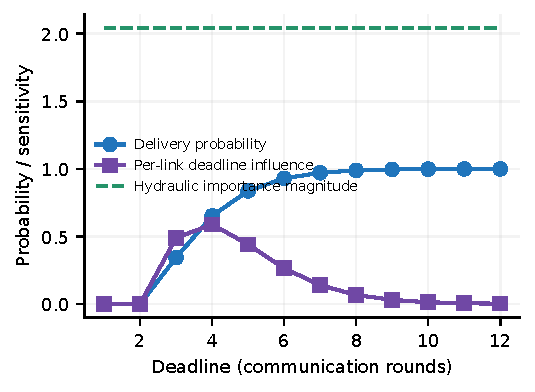
\includegraphics[width=\columnwidth]{figures/deadline_example.pdf}
\caption{An exact three-hop example separates persistent-flow importance from
deadline sensitivity. One report originates before the first round; each round
allows one forwarding hop. Curves are analytical, not additional USV trials.
The electrical analogy assigns importance even when timely delivery is impossible.}
\label{fig:deadline_example}
\end{figure}

\subsection{Limits of the biological interpretation}
The fungal implementation transfers a division of functions: spatial expansion,
transport reinforcement and rejection of redundant expenditure. It does not
simulate fungal tissue, consume construction material, reproduce a travelling
wave, or inherit the biological model's near-Pareto behavior. Ant recruitment
transfers activity-dependent participation; it does not establish that a
liquid-brain mechanism is necessary or best for radio-linked vessels.
Biology is therefore a source of falsifiable proposal mechanisms.

Failure to beat a conventional matched control is scientifically informative.
The coupled activity can preserve a useful role allocation under noisy
observations, but it can also delay a needed change or allocate work according
to obsolete conditions. A global performance gain does not identify the
social term as causal without its ablation. More neuron-like dynamics,
spiking models or evolutionary tuning would introduce additional hypotheses;
none should be added solely to make the method sound more sophisticated.

\subsection{What must be calibrated before deployment}
Three gaps dominate the distance between these results and practical use.
First, sensor curves must come from known objects, ranges and environmental
conditions, with detection and false-alarm definitions fixed in advance.
Availability and range should be estimated jointly; a sequence of distant
misses is often uninformative about which one degraded. An intervention that
improves parameter estimation is worthwhile only if its expected mission value
exceeds its cost. Information gain alone is not that value.

Second, radio tests need packet timestamps, retries, traffic load, antenna
geometry and common-outage measurements. The present ideal cache network has
no finite throughput; 192 virtual monitoring points do not imply a measured
192-object traffic load. A realistic network extension should test
finite-capacity scheduling and distinguish direct base delivery, relay
delivery and command acknowledgement.

Third, a fitted marine dynamics model should predict the energy and timing of
station keeping and formation changes. The present power law,
$60+18|u|^3+8v^2+4r^2$ W, is a declared synthetic model.
Replacing it by vessel-specific hydrodynamics and actuator data could change
the preferred formation policy. A marine-craft model provides an appropriate
structure for that work~\cite{fossen2021}.
Near-field repulsion and sampled separation checks are not COLREGs reasoning,
formal safety filters or evidence of seaworthiness.

\subsection{A bounded route to stronger mathematics}
The original requirement also needs a distinction between continuous graph
connectivity and timely delivery. These experiments improve delivered freshness;
they do not enforce an always-connected graph. Let $\mathcal E_D(g)$ denote the
event that every required vessel has a causal path to the base within $D$.
A future constrained controller could require a calibrated lower bound on
$\Prb\{\mathcal E_D(g)\}$ to exceed $1-\alpha$, or impose an explicit instantaneous connectivity constraint
when that is the actual mission requirement. Such a problem needs feasibility
handling: under a total blackout, a positive reliability requirement is
infeasible. An appropriate fallback would report the outage and preserve local
data, rather than treat the constraint as satisfied. This constraint and its
calibration are proposed future work, not implemented guarantees.

The next mathematical extension should attach a model-error allowance to
the acceptance decision. If, for every compared action,
$|\widehat J(g)-J^\star(g)|\leq\delta$, then accepting only when
$\widehat J(g)-\widehat J(g_0)>2\delta$ ensures a positive difference in
$J^\star$. This follows directly from two applications of the error bound.
The difficult research task is obtaining a valid $\delta$ under delayed
telemetry, health uncertainty and model mismatch. The present implementation
does not possess such a bound.

One practical route is a separately calibrated probability model and an
independent rollout bank for candidate validation. A confidence interval for a
sample average only controls integration error under the assumed model; it
does not cover unmodeled radio interference or sensor clutter.
Distributionally robust planning or calibrated ambiguity sets could address
part of that gap. Such an extension should be compared with a conventional
robust local controller using the same information and uncertainty budget.

To scale the deadline-fusion calculation, cache backward-reachability states
and skip edge-round interventions that cannot alter useful source reachability.
The exact finite-network enumeration test provides a regression oracle for
that optimization. A faster implementation with preserved conditional
expectations would be a concrete addition, even if the biological interpretation
itself does not improve fleet-level outcomes.

\subsection{Learning as a controlled extension}
Learning should address a residual choice that the model-based controller
cannot set well across conditions: step length, energy price, forecast horizon
or a small proposal mixture. Observation history can help infer persistent
degradation from delayed measurements. The released residual adapter exposes
cached per-vessel geometry, belief moments, ages, energy, previous waypoint
errors and global mission context. It adds no hidden-health observation.

A linear history policy is intentionally a transparent baseline. More training
does not guarantee it will outperform the fixed economic rule.
The short PPO study in Section~\ref{sec:v4} adds multiple training seeds and constant-setting controls. A subsequent PPO or recurrent-policy experiment should compare one versus four observations,
domain randomization on/off, multiple training seeds and the best constant
residual action selected on development data. Its evaluation must retain the
movement and communication constraints. Success on a training reward or a
single checkpoint is insufficient evidence of practical learning value.

\subsection{Publication position}
This package is a reproducible simulation manuscript with explicit hypotheses,
negative comparisons and inspectable mathematics. It is ready to be reviewed
and versioned as a research repository. It is not evidence of journal acceptance
or of first use of these ideas in robotics. A journal-strength next version
should make one narrow claim, reproduce closer optimization baselines, and
validate a relevant physical model or hardware-in-the-loop implementation.
For an internship, the strongest immediate product is the measured
coverage--energy decision workflow and the experiments it makes possible.

\section{Conclusion}
Formation adaptation should be evaluated at the receiver, with physical movement
costs and causal report delivery included. This study supplies a common economic
controller, biologically motivated proposal families and a deadline-sensitive
link-importance transfer, evaluated against development-selected static geometry
and conventional controls. The economic controller achieves the clearest
coverage--energy improvement over the earlier adaptive architecture. The small
pooled biological gains are not robust across the diagnostic settings, and the
first evaluated residual learner does not improve the mission objective.
The deadline-influence formulation remains an inspectable research mechanism,
not an established performance breakthrough. The next practical step is calibration and validation of the
sensing, channel and movement models, followed by a fresh held-out comparison.
